% Name: Elliptical orbit
% Description: A planet on an ellipse of eccentricity 0.6 with the Sun at one focus: the semi-major and semi-minor axes, perihelion and aphelion, the pull toward the Sun, and the velocity along the tangent.
% Tags: orbit, Kepler's laws, ellipse, gravitation

\usetikzlibrary{arrows.meta, shapes.misc}

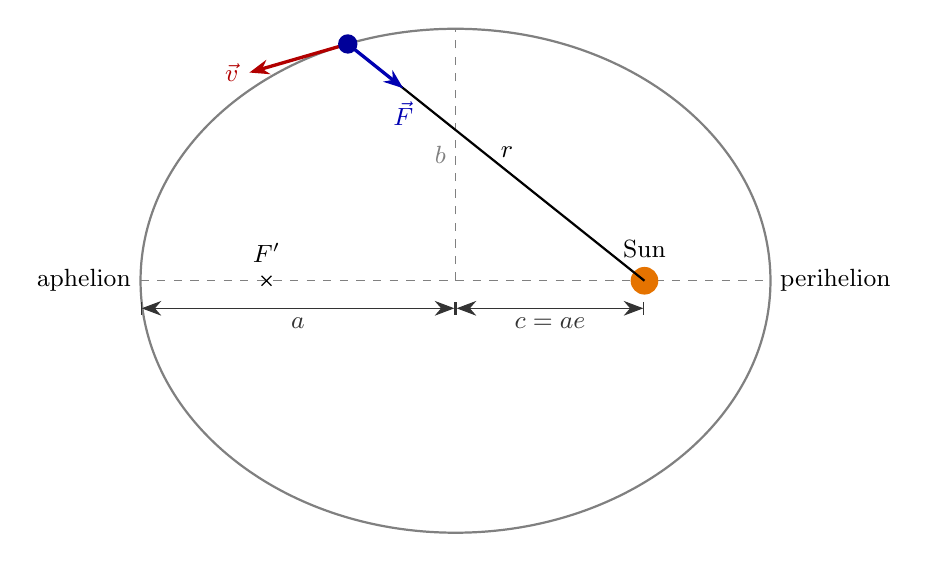
\begin{tikzpicture}[>={Stealth[length=2.5mm]}, every node/.style={font=\small}]
  % a = 4, e = 0.6, so c = ae = 2.4 and b = a sqrt(1 - e^2) = 3.2; the planet sits at the parameter t = 110 degrees.
  \draw[thick, gray] (0,0) ellipse[x radius=4, y radius=3.2];
  \draw[dashed, gray] (-4,0) -- (4,0);
  \draw[dashed, gray] (0,0) -- node[left] {$b$} (0,3.2);
  \draw[|<->|, gray!40!black] (-4,-0.35) -- node[below] {$a$} (0,-0.35);
  \draw[|<->|, gray!40!black] (0,-0.35) -- node[below] {$c = ae$} (2.4,-0.35);
  \fill[orange!90!black] (2.4,0) circle (5pt) node[above=5pt, black] {Sun};
  \draw (-2.4,0) node[cross out, draw, inner sep=1.6pt] {} node[above=3pt] {$F'$};
  \node[right] at (4,0) {perihelion};
  \node[left] at (-4,0) {aphelion};
  \coordinate (P) at ({4*cos(110)},{3.2*sin(110)});
  \draw[thick] (2.4,0) -- node[above right=-2pt] {$r$} (P);
  % Tangent (-4 sin t, 3.2 cos t) normalized is (-0.960, -0.279); toward the Sun the unit vector is (0.782, -0.624).
  \draw[->, very thick, red!70!black] (P) -- ++(-1.25,-0.363) node[left] {$\vec{v}$};
  \draw[->, very thick, blue!70!black] (P) -- ++(0.704,-0.562) node[below=1pt] {$\vec{F}$};
  \fill[blue!60!black] (P) circle (3.5pt);
\end{tikzpicture}
